\documentclass[11pt]{amsart}

\usepackage{lmodern}
\usepackage[T1]{fontenc}
\usepackage{amsmath,amssymb,amsthm}
\usepackage{mathrsfs}
\usepackage{tikz}
\usepackage{listings}
\usepackage[margin=1in]{geometry}
\usepackage{microtype}
\usepackage[hidelinks]{hyperref}

\lstset{
  basicstyle=\ttfamily\small,
  columns=fullflexible,
  keepspaces=true,
  showstringspaces=false,
  language=Python,
  breaklines=true,
  frame=none,
  aboveskip=1ex,
  belowskip=1ex
}

\theoremstyle{plain}
\newtheorem{theorem}{Theorem}[section]
\newtheorem{proposition}[theorem]{Proposition}
\newtheorem{corollary}[theorem]{Corollary}
\theoremstyle{definition}
\newtheorem{definition}[theorem]{Definition}
\newtheorem{remark}[theorem]{Remark}

\newcommand{\Ok}{\mathscr{O}_k}
\newcommand{\Onum}[1]{\mathscr{O}_{#1}}
\newcommand{\Q}{\mathbb{Q}}
\newcommand{\R}{\mathbb{R}}
\newcommand{\code}[1]{\texttt{#1}}

\setlength{\emergencystretch}{3em}

\begin{document}

\title{Regular Polygons and a Hierarchy of Origami Numbers}
\author{Charles C. Norton}
\address{Long Island, New York}
\email{cnorton2@binghamton.edu}
\date{July 2026}
\subjclass[2020]{Primary 51M15, 12F10; Secondary 11R18, 68V20}
\keywords{origami constructions, multifold origami, regular polygons, Euler totient, Gaussian periods, Galois theory, interactive theorem proving}

\begin{abstract}
For each $k \ge 1$, let $\Ok$ be the field generated by the $k$-crease coupled Lill fold: the closure of the rationals under field operations, square roots, and real roots of monic polynomials of prime degree at most $2k+1$. We prove that for $n \ge 3$, the regular $n$-gon lies in $\Ok$ if and only if every prime factor of $\varphi(n)$ is at most $2k+1$. The characterization is exact in both directions and new for every $k \ge 2$; the impossibility direction is, to our knowledge, the first for any hierarchy of multifold origami numbers, and the classical single-fold theorem is the base instance $\Onum{1}$. The constructive direction runs a real Gaussian-period tower over an unconditional primitive root, with Chebyshev recurrences at prime powers and a B\'ezout reduction at composites; the impossibility direction is a smooth degree bound against the exact cosine degree $\varphi(n)/2$. The substrate is a coupled Lill fold in which $k$ simultaneous creases solve an arbitrary monic polynomial of degree $2k+1$, one crease per two degrees against the classical Lill rate of one per degree. Unrestricted multifold origami is larger and far less understood: two folds alone already construct every polygon of $\Onum{3}$, through the angle septisection of K\"onig and Nedrenco and its lower-degree predecessors, yet no impossibility is known for it and its exact reach is open. The cleanly generated hierarchy $\Ok$ is where an exact characterization is available. Every numbered theorem and corollary is machine-checked in the Rocq prover, and the development is publicly available. Three short Python programs demonstrate the arithmetic numerically.
\end{abstract}

\maketitle

\section{Introduction}

Which regular polygons can be folded? The single-fold answer is classical. The Huzita--Justin--Hatori axioms generate, beyond ruler and compass, the real roots of cubics with constructible coefficients: Gleason \cite{gleason} observed that angle trisection extends the compass polygons to those with $2$-$3$-smooth totient, and Alperin \cite{alperin} identified the resulting field of origami numbers. The regular $n$-gon is single-fold constructible exactly when every prime factor of $\varphi(n)$ is $2$ or $3$; equivalently, when $n = 2^a 3^b$ times a product of distinct Pierpont primes \cite{pierpont}.

Multifold origami, in which several creases are formed simultaneously, each constrained by alignments possibly referring to the others, extends the reach. Alperin and Lang \cite{alperinlang} introduced the multifold axiom framework and, through Lill's method \cite{hull}, showed that a polynomial of degree $m$ can be solved with $m-2$ simultaneous creases. Two-fold origami solves quintics (Nishimura \cite{nishimura}, Lucero \cite{luceroquintic}) and even septics (K\"onig and Nedrenco \cite{koenig}). For polygons, Lucero \cite{lucero} proved the general sufficiency result: the regular $m$-gon is $n$-fold constructible if the largest prime factor of $\varphi(m)$ is at most $n+2$, noting explicitly that the conditions are sufficient only. No impossibility result at any multifold level has appeared.

This paper characterizes exactly, in both directions and under machine verification, the regular polygons of the graded hierarchy generated by Lill's method. Our contributions:

\begin{enumerate}
\item \textbf{A faster Lill fold.} A system of $k$ simultaneous creases coupled in a chain by $k-1$ common perpendiculars is sound over every monic polynomial of degree $2k+1$ with constructible coefficients (each configuration yields a real root), and realizes every root of the Bring--Jerrard family $t^{2k+1}+pt+q$. Each added crease raises the solvable degree by two, against one for the classical multifold Lill rate.

\item \textbf{The exact characterization.} With $\Ok$ the field this operation generates (Definition~\ref{def:onk}), the regular $n$-gon lies in $\Ok$ \emph{if and only if} every prime factor of $\varphi(n)$ is at most $2k+1$ (Theorem~\ref{thm:main}). The $k=1$ instance is Alperin's field of single-fold origami numbers; $k=2$ and $k=3$ are the closures under the quintic and septic Lill folds. The impossibility direction is, to our knowledge, the first for any hierarchy of multifold origami numbers. Its technical core is a smooth degree bound (Theorem~\ref{thm:degbound}) that survives the absence of irreducibility in the class's root constructor: because a nominal degree-$d$ step need not be a degree-$d$ field extension, the tower law does not apply directly, and the actual step degree must be pinned through the maximal independent prefix of the powers of the adjoined element. This bound, not the mere existence of a multifold field, is what forces the totient condition.

\item \textbf{Machine verification.} Every theorem stated here is proved in the Rocq prover (formerly Coq), in a development whose mathematical core assumes exactly the four standard classical axioms of real analysis and contains no admitted proofs \cite{repo}. The paper presents the mathematical content; the formalization carries the full detail, and we cite the formal theorem names throughout.
\end{enumerate}

Unrestricted multifold origami, with several creases in general position, is the wider setting, and a difficult one. By Gleason's reduction \cite{gleason} a regular $n$-gon is constructible once every prime factor of $\varphi(n)$ can be angle-multisected; K\"onig and Nedrenco \cite{koenig} septisect an arbitrary angle with two folds, and with quintisection \cite{nishimura, luceroquintic} and the classical trisection this places every polygon of $\Onum{3}$ within reach of unrestricted two-fold origami (Theorem~\ref{thm:main} at $k=3$). Yet no impossibility is known for the unrestricted class beyond the single-fold case, and whether a totient criterion governs it at all is open (Section~\ref{sec:outlook}). The hierarchy $\Ok$ generated by the coupled Lill fold is the tractable part of this landscape: it is cleanly defined, both directions are available, and the level of a polygon in it is the reach of the Lill fold, which Theorem~\ref{thm:main} determines exactly. Within that scope Remark~\ref{rem:robust} shows the criterion is even insensitive to a natural enlargement of the class.

\section{The hierarchy of $k$-fold origami numbers}

\begin{definition}\label{def:onk}
For $k \ge 1$, the class $\Ok \subseteq \R$ (formal name \code{OrigamiNumK k}) is defined inductively: it contains $0$ and $1$; it is closed under addition, subtraction, multiplication, and inverses of nonzero elements; it is closed under square roots of nonnegative elements; and for every prime $d \le 2k+1$, it is closed under real roots of monic degree-$d$ polynomials with coefficients in $\Ok$ (constructor \code{ONK\_proot}: if $c_0,\dots,c_{d-1} \in \Ok$ and $r^d + c_{d-1}r^{d-1} + \cdots + c_0 = 0$, then $r \in \Ok$).
\end{definition}

\begin{proposition}[\code{OrigamiNumK\_1\_iff}, \code{OrigamiNumK\_2\_iff}, \code{OrigamiNumK\_3\_iff}]\label{prop:levels}
$\Onum{1}$ is Alperin's field of origami numbers; $\Onum{2}$ and $\Onum{3}$ are the closures under the quintic and septic Lill folds.
\end{proposition}

Three elementary structural remarks will be needed.

\begin{remark}[grading by primes]\label{rem:grading}
$\Ok = \Onum{k+1}$ unless $2k+3$ is prime: the constructors of the two classes differ only in the admitted prime degrees. In particular $\Onum{3} = \Onum{4}$, since the primes at most $9$ are the primes at most $7$. The hierarchy steps exactly at the odd primes.
\end{remark}

\begin{remark}[no irreducibility, and a padding bound]\label{rem:padding}
The root constructor imposes no irreducibility on the witnessing polynomial. Consequently, any real algebraic number of degree $m$ lies in $\Ok$ as soon as some prime $d$ with $m \le d \le 2k+1$ exists: multiply the minimal polynomial by $(x-a)^{d-m}$ for any $a \in \Ok$ and apply the constructor. Membership in $\Ok$ is therefore \emph{not} a condition on degrees alone, and upper bounds on the hierarchy must be argued through towers, as in Theorem~\ref{thm:degbound}.
\end{remark}

\begin{remark}[strictness]\label{rem:strict}
The chain $\Onum{1} \subseteq \Onum{2} \subseteq \cdots$ of polygon sets is strict at every prime $p = 2k+1 \ge 5$: $\varphi(p^2) = p(p-1)$ has largest prime factor exactly $p$, so by Theorem~\ref{thm:main} the $p^2$-gon lies in $\Onum{k}$ and not $\Onum{k-1}$. The $25$-gon enters at $\Onum{2}$, the $49$-gon at $\Onum{3}$, and the $121$-gon at $\Onum{5}$, each together with its non-membership one level below machine-checked (\code{rem\_2\_3\_strict\_25}, \code{rem\_2\_3\_strict\_49}, \code{rem\_2\_3\_strict\_121}); the $9$-gon separates nothing, since $\varphi(9)=6$ is already $3$-smooth and there is no tier below $k=1$.
\end{remark}

\section{The geometric substrate: $k$ coupled creases solve degree $2k+1$}\label{sec:geom}

Lill's method represents a monic polynomial as a right-angle path and recovers a root from a reflecting path between its endpoints; Beloch's fold is the case of the cubic, where the reflecting path is produced by one crease tangent to two parabolas \cite{hull}. The classical multifold generalization requires one crease per additional degree: $m-2$ simultaneous creases for degree $m$ \cite{alperinlang, lucero}.

The coupled system improves this rate. For a monic polynomial of degree $2k+1$ with coefficients $a_0,\dots,a_{2k}$ in a field of constructible coordinates, place the alternating Lill coefficient lines and form $k$ creases $g_1,\dots,g_k$ subject to: each $g_i$ passes through the two incidence points demanded by Lill's bounce at its station, consecutive creases are coupled by common perpendicular bounce segments, and a terminal perpendicular closes the path. Each crease absorbs \emph{two} reflections of the Lill path rather than one. The reflecting path of a degree-$(2k+1)$ polynomial runs in $2k+1$ segments and turns $2k$ times at its interior vertices, and the coupling lets each crease effect two of those turns, so $k$ creases account for all $2k$. This is why an added crease buys two degrees where a single fold buys one, and the solvable degree is $2k+1$ rather than $k+2$: at $k=1$ the two rates meet at the cubic (Beloch's fold), and the gain opens from $k=2$ onward.

These constraints are the two alignment primitives of the Huzita--Alperin--Lang framework \cite{alperinlang, hull}: incidence of a crease with constructed points, and perpendicularity of a crease to a reference line through a point. Both are Huzita folds, and the identification is formal. The incidence line through two points is the fold O1: its crease is exactly \code{line\_through} (companion \code{fold\_O1\_line\_through}). The perpendicular is the fold O4: its crease is perpendicular to the reference line and passes through the point (companion \code{fold\_O4\_perp\_incident}). A $k$-fold operation forms $k$ such creases simultaneously, the alignments holding jointly (the coupling across creases being what single folds cannot do), and Theorem~\ref{thm:realizable} exhibits, for each root, an explicit configuration meeting them.

\begin{theorem}[\code{general\_lill\_solves}]\label{thm:lill}
Every configuration of the $k$ coupled creases over the coefficient lines of a monic degree-$(2k+1)$ polynomial produces a real root of that polynomial.
\end{theorem}

\begin{theorem}[\code{k\_fold\_lill\_realizable}]\label{thm:realizable}
Conversely, in the Bring--Jerrard family $t^{2k+1} + pt + q$ with $q \ne 0$, every real root $t$ is realized by an explicit configuration: the $k$ mirrors of normal $(1,-t)$ given by $x - ty = 1 + (-1)^i t^{2i+2}$, with the bounce path alternating between the line $x=1$ and the $x$-axis. Figure~\ref{fig:lill} shows the $k=2$ system at $(p,q) = (-3,1)$.
\end{theorem}

\begin{figure}[ht]
\centering
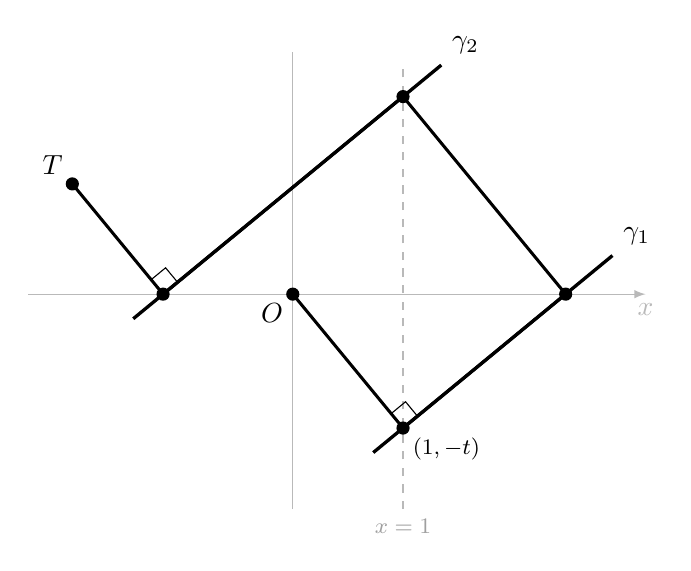
\begin{tikzpicture}[scale=1.4]
  % axes
  \draw[gray!55,-latex] (-2.4,0) -- (3.2,0) node[below] {$x$};
  \draw[gray!55] (0,-1.95) -- (0,2.2);
  % alignment line x = 1, touched by the path at (1,-t) and (1,t^3); label at bottom
  \draw[gray!55,dashed] (1,-1.95) -- (1,2.1);
  \node[gray!75,below] at (1,-1.95) {\footnotesize $x=1$};
  % the two creases: parallel, both of normal (1,-t); the middle bounce segments run along them
  \draw[very thick] (0.730,-1.437) -- (2.900,0.350) node[above right] {$\gamma_1$};
  \draw[very thick] (-1.447,-0.223) -- (1.347,2.078) node[above right] {$\gamma_2$};
  % bounce path O -> (1,-t) -> (1+t^2,0) -> (1,t^3) -> (1-t^4,0) -> T
  \draw[line width=1.1pt]
    (0,0) -- (1,-1.2146) -- (2.4754,0) -- (1,1.7921) -- (-1.1767,0) -- (-2,1);
  % right-angle marks where connectors meet the creases perpendicularly
  \draw[thin] (0.892,-1.084) -- (1.023,-0.976) -- (1.131,-1.107);
  \draw[thin] (-1.045,0.108) -- (-1.154,0.239) -- (-1.285,0.131);
  % vertices
  \foreach \p in {(0,0),(1,-1.2146),(2.4754,0),(1,1.7921),(-1.1767,0),(-2,1)}
    \fill \p circle (1.7pt);
  \node[below left] at (0,0) {$O$};
  \node[above left] at (-2,1) {$T$};
  \node[below right] at (1,-1.2146) {\footnotesize $(1,-t)$};
\end{tikzpicture}
\caption{The two-crease coupled Lill system solving $t^5 - 3t + 1 = 0$ at the real root $t \approx 1.2146$. The bounce path from $O$ to $T = (p+1,q)$ folds along the creases $\gamma_1,\gamma_2$, both of normal $(1,-t)$; the connecting segments meet the creases at right angles (the couplings), and the terminal segment to $T$ is perpendicular to $\gamma_2$.}\label{fig:lill}
\end{figure}

The same family admits a second crease presentation, one Beloch step per crease: the pencil crease $\{t,-1,-t^{2k}\}$, of normal $(t,-1)$, reflects the point $(q,p)$ onto the line $x=-q$ exactly when $t^3 + pt + q = 0$ (Beloch, $k=1$), and the $k$-crease chain does the same at degree $2k+1$ (\code{k\_fold\_lill\_solves}; the $k=2$ and $k=3$ instances, with full closure of the crease coordinates in $\Onum{2}$ and $\Onum{3}$, are \code{twofold\_reflects\_quintic} and \code{three\_fold\_lill\_septic}). Program~3 below verifies the incidence identity numerically at degrees $3$, $5$, and $7$.

Since every prime $d \le 2k+1$ is either $2$ (a single fold) or odd with $(d-1)/2 \le k$ creases, each root constructor of Definition~\ref{def:onk} corresponds to a $k$-crease fold of the matching degree, and Theorem~\ref{thm:lill} certifies its soundness: every such fold configuration produces a root of the polynomial it is built over. Two boundaries of the geometric grounding are worth stating exactly. \emph{Realizability}, meaning that a \emph{prescribed} constructor root is met by some configuration (the converse of Theorem~\ref{thm:lill}), is established for the Bring--Jerrard family $t^{2k+1}+pt+q$ at every $k$ (Theorem~\ref{thm:realizable}), and for all of $\Onum{2}$ and $\Onum{3}$ at $k \le 3$, where Proposition~\ref{prop:levels} identifies the classes and the crease coordinates are proved to lie in them. \emph{Conservativity}, meaning that the coupled fold produces nothing outside $\Ok$, is likewise a $k \le 3$ theorem, and is expected at every $k$ for a structural reason: $\Ok$ is defined to admit exactly the roots the fold produces. A degree-$(2k+1)$ configuration yields, by Theorem~\ref{thm:lill}, a real root of a monic polynomial in its already-constructed coefficient data, which is precisely the closure the constructor \code{ONK\_proot} imposes; what the $k \le 3$ theorems add is that the auxiliary crease coordinates lie in the class as well, and no new mechanism enters at higher degree. At higher $k$ we therefore take Definition~\ref{def:onk} as the definition of $\Ok$: the conservative class the $k$-crease operation is guaranteed to reach, grounded geometrically at $k \le 3$ and by soundness and Bring--Jerrard realizability at all $k$. None of this bears on the main theorem, whose sufficiency (Theorem~\ref{thm:main}) is purely algebraic and never invokes realizability; and Remark~\ref{rem:robust} shows the polygon criterion is insensitive to the remaining modeling choices.

\section{The main theorem}

\begin{theorem}[\code{ngon\_k\_fold\_iff}]\label{thm:main}
Let $k \ge 1$ and $n \ge 3$. Then $\cos(2\pi/n) \in \Ok$ if and only if every prime factor of $\varphi(n)$ is at most $2k+1$.
\end{theorem}

Equivalently, in arithmetic form: the regular $n$-gon lies in $\Ok$ iff $n = 2^{a_0} q_1^{a_1} \cdots q_s^{a_s}\, p_1 \cdots p_r$, where the $q_i \le 2k+1$ are primes appearing to arbitrary powers and the $p_j > 2k+1$ are distinct primes with each $p_j - 1$ being $(2k+1)$-smooth. At $k=1$ the $p_j$ are the Pierpont primes.

\subsection{Sufficiency}

Fix $k$ and $n$ with $\varphi(n)$ $(2k+1)$-smooth. Write $n = q^e \cdot m$ with $q$ prime, $q \nmid m$, and induct on $n$ (\code{cos\_sin\_smoothK}).

\emph{Composites.} If $m > 1$, then $\gcd(q^e, m) = 1$ and $\varphi(n) = \varphi(q^e)\varphi(m)$, so both factors inherit smoothness. With $ua - vb = 1$ a B\'ezout relation between the coprime parts, $2\pi/n = u(2\pi/b) - v(2\pi/a)$; the cosine and sine addition laws pass constructibility of $\cos$ and $\sin$ at both denominators to the product (\code{cos\_sin\_ONK\_mul}), and $\sin$ is recovered from $\cos$ as $\sqrt{1-c^2}$ (\code{sin\_ONK\_of\_cos}).

\emph{Prime powers.} $\cos(2\pi/q^e)$ is a root of the monic prime-degree-$q$ polynomial $(T_q(x) - \cos(2\pi/q^{e-1}))/2^{q-1}$, where $T_q$ is the Chebyshev polynomial; its coefficients lie in the class by induction on $e$, and $q \le 2k+1$ by smoothness, so the root constructor applies (\code{cos\_2pi\_qe\_ONK}, with the coefficient list \code{cheb\_coeffs} and its top coefficient $2^{q-1}$ handled explicitly).

\emph{Primes.} For prime $p \ge 5$, let $g$ be a primitive root mod $p$. Its existence is proved unconditionally, with no smoothness hypothesis, by assembling an element of order $p-1$ from elements of coprime prime-power orders, by strong induction over the unitary divisors of $p-1$ (\code{primitive\_root\_gen}). The real Gaussian periods over $\langle g \rangle$ give a tower $\Q = K_0 \subset K_1 \subset \cdots \subset K_r \ni 2\cos(2\pi/p)$ whose successive degrees are the prime factors $\rho$ of $p-1$, each $\le 2k+1$ by smoothness. At each rung, Newton's identities express each elementary symmetric function of the finer periods as an integer-coefficient combination of their power sums divided by an integer; in characteristic zero this recovers the symmetric functions from the power sums, keeping them in the level $K$, and Vieta then presents each finer period as a root of a monic degree-$\rho$ polynomial over $K$ (\code{esym\_K}, \code{step\_prime\_K}, \code{tower\_cos\_prime\_rungs}). Every rung is one application of the root constructor. \qed

\subsection{Necessity}

The necessity direction does not follow formally from the existence of a multifold field: it turns on the degree bound of Theorem~\ref{thm:degbound}, whose proof is the technical core of the impossibility side. The subtlety is that the root constructor of Definition~\ref{def:onk} admits \emph{non-irreducible} witnessing polynomials (Remark~\ref{rem:padding}), so a tower step $F \subset F[r]$ of nominal degree $d$ need not have field degree $d$, and the na\"ive tower law does not apply. The bound is recovered instead through the maximal linearly independent prefix of the powers of $r$, which pins the actual step degree to a value between $1$ and $d$ while preserving the smoothness of the product. The mechanism is elementary. The monic relation expresses $r^d$, and by iterated multiplication by $r$ and reduction every higher power, as an $F$-combination of $1, r, \dots, r^{d-1}$, so these $d$ powers span $F[r]$ regardless of whether the relation factors. The first power $r^j$ that becomes dependent on its predecessors renders every later power dependent as well, so the longest independent prefix $1, \dots, r^{j-1}$ already spans: it is a basis, of length $j \le d$. That length is a genuine field-extension degree, at most $2k+1$; irreducibility would only force $j = d$, and the smooth bound needs none of it. The tower law then multiplies these true degrees, and no prime exceeding $2k+1$ can divide the product.

\begin{theorem}[exact cosine degree, \code{cos\_2pi\_n\_degree\_exactly}]\label{thm:cosdeg}
For $n \ge 3$, $[\Q(2\cos(2\pi/n)) : \Q] = \varphi(n)/2$. This is the classical degree of the maximal real subfield of the $n$-th cyclotomic field; it rests on the irreducibility of the $n$-th cyclotomic polynomial for all $n$ (composite included), the standard Dedekind result, proved here by reduction modulo a prime with the Dedekind--Frobenius argument and machine-checked in \code{cyclotomic.v} rather than assumed.
\end{theorem}

\begin{theorem}[smooth degree bound, \code{OrigamiNumK\_field\_degree\_smooth}]\label{thm:degbound}
Every $x \in \Ok$ has finite degree over $\Q$, and every prime factor of that degree is at most $2k+1$.
\end{theorem}

\begin{proof}[Proof sketch]
Each $x \in \Ok$ lies at the top of a finite tower over $\Q$ whose steps are either quadratic or of the form $F \subset F[r]$ with $r$ satisfying a monic relation of degree $d \le 2k+1$ over $F$ (\code{ONK\_in\_oktower}; the relation need not be irreducible). Each step is spanned by the maximal linearly independent prefix of the powers $1, r, \dots, r^{d-1}$, a basis of size between $1$ and $d$ (\code{powers\_max\_prefix}, \code{PolyF\_step\_basis}). By the tower law the degree of $x$ divides a product of step sizes each at most $2k+1$ (\code{oktower\_dim}, \code{tower\_law\_div}), and every prime factor of such a product is at most $2k+1$.
\end{proof}

Now suppose $\cos(2\pi/n) \in \Ok$ and some prime $P > 2k+1$ divides $\varphi(n)$. Then $2\cos(2\pi/n) \in \Ok$, its degree is $\varphi(n)/2$ by Theorem~\ref{thm:cosdeg}, and $P$, odd since $P > 2k+1 \ge 3$, divides $\varphi(n)/2$, contradicting Theorem~\ref{thm:degbound} (\code{cos\_2pi\_n\_not\_k\_fold}). \qed

\begin{remark}[robustness of the polygon criterion]\label{rem:robust}
Theorem~\ref{thm:degbound} is formalized for towers whose steps have \emph{arbitrary} degree $d$ with $2 \le d \le 2k+1$; primality is nowhere used on the necessity side (\code{okwf} imposes only the bound). Consequently, enlarging $\Ok$ by composite-degree root steps up to $2k+1$ (for instance admitting the degree-$9$ coupled Lill system at $k=4$, where $2k+1$ is not prime) changes no polygon's level: sufficiency uses only prime rungs, and the degree bound is unaffected. The criterion is therefore independent of these modeling choices.
\end{remark}

\subsection{Corollaries}

\begin{corollary}[minimal level, \code{cor\_4\_5\_closed\_form}, \code{cor\_4\_5\_minimal\_budget}]\label{cor:budget}
For $n \ge 3$, the least $k$ with $\cos(2\pi/n) \in \Ok$ is $k(n) = \lfloor P/2 \rfloor$, where $P$ is the largest prime factor of $\varphi(n)$: the $n$-gon lies in $\Onum{\lfloor P/2 \rfloor}$ and in no $\Onum{j}$ below it (\code{cor\_4\_5\_closed\_form}, the arithmetic $2\lfloor P/2\rfloor + 1 \ge P > 2j+1$ discharged against the smoothness threshold). Equivalently, $k$ is the least level iff $2k+1$ is the smoothness threshold of $\varphi(n)$, smooth at $2k+1$ and not below (\code{cor\_4\_5\_minimal\_budget}).
\end{corollary}

\begin{corollary}[first polygons]\label{cor:first}
The $11$-gon is the first polygon to enter at $\Onum{2}$, its quintic realized concretely by Lucero \cite{luceroeleven}; the $29$-gon is the first to enter at $\Onum{3}$; the $23$-gon the first at $\Onum{5}$, with $\Onum{4} = \Onum{3}$ by Remark~\ref{rem:grading}; the $47$-gon enters at $\Onum{11}$. Lucero's $199$-gon \cite{lucero}, which his sufficiency bound places at nine folds, enters at $\Onum{5}$, since $\varphi(199) = 2 \cdot 3^2 \cdot 11$. Each of these five entry levels (membership at the stated level and at none below) is machine-checked (\code{cor\_4\_6\_hendecagon} through \code{cor\_4\_6\_199gon}), together with three threshold facts: every polygon below the $11$-gon lies in $\Onum{1}$, every polygon below the $29$-gon lies in $\Onum{2}$ or outside $\Onum{3}$, and every polygon below the $23$-gon lies in $\Onum{4}$ (\code{cor\_4\_6\_first\_two\_fold}, \code{cor\_4\_6\_first\_exactly\_three}, \code{cor\_4\_6\_first\_five}).
\end{corollary}

\begin{remark}[levels and simultaneous folds]\label{rem:physical}
The level $k(n)$ of Corollary~\ref{cor:budget} is the reach of the coupled Lill fold, and it equals the number of simultaneous folds physically required only at the bottom of the hierarchy. At $k=1$ it is Alperin's single-fold constructibility. At the hendecagon it again coincides with the true count: a single fold constructs no number of degree $5$, whereas $2\cos(2\pi/11)$ has degree $5$ over $\Q$, and two folds reach it, so the $11$-gon requires exactly two simultaneous folds and is the one polygon in this range whose $\Ok$-level is its physical fold count. Above the hendecagon the two part company. Two unrestricted folds already reach every polygon of $\Onum{3}$ (Section~\ref{sec:outlook}), so for $n$ entering at $\Onum{3}$ or beyond the level bounds the simultaneous-fold requirement from above without meeting it. Theorem~\ref{thm:main} is a statement about the field $\Ok$; its reading as a fold count is exact only where the two agree.
\end{remark}

\begin{corollary}[exhaustion, \code{cor\_4\_7\_exhaustion}]\label{cor:exhaust}
$\bigcup_k \Ok$ contains $\cos(2\pi/n)$ for every $n$: every regular polygon lies in some $\Ok$, and its minimal level is determined by a single prime.
\end{corollary}

\section{Verification in Rocq}

The development \cite{repo} is carried out in Rocq~9 over its standard library. The results of this paper are collected in a single companion file, \code{theories/kfold\_ngon.v}, which restates each numbered theorem under a paper-facing name (the main theorem as \code{thm\_4\_1\_kfold\_ngon}, and so on), discharges it by the corresponding theorem of the development, proves the axiom-bridge lemmas of Section~\ref{sec:geom}, the strictness witnesses of Remark~\ref{rem:strict}, and every corollary of Section~4.3 (the minimal-level characterization, the five first-polygon levels with the three threshold facts, and exhaustion), type-checks the supporting lemmas named in the proof sketches, and prints the axiom footprint of the main theorem. The underlying proofs are distributed over \code{theories/foundations.v} (algebra, polynomials, linear algebra, the degree theory), \code{theories/cyclotomic.v} (roots of unity, cyclotomic irreducibility for all $n$, Chebyshev polynomials, the exact cosine degree), \code{theories/geometry.v} (the fold axioms, the class \code{OrigamiNumK}, and \code{ngon\_k\_fold\_iff}), and \code{theories/frontier.v} (the coupled Lill systems of Section~\ref{sec:geom}). \code{Print Assumptions} on the main theorem reports exactly four axioms (excluded middle, dependent functional extensionality, and the two decidability axioms underlying the classical construction of the reals in the standard library) with no admitted proofs; the discrete layer (integers, polynomials, cyclotomic arithmetic) is axiom-free. Each proof given above is a summary of the corresponding machine-checked argument, which contains the complete detail.

\section{Numerical demonstrations}

Three programs, using only the standard library, illustrate the arithmetic of the theorem; the proofs are in \cite{repo}.

\medskip
\noindent\textbf{Program 1: the minimal level.} An implementation of Corollary~\ref{cor:budget}.

\begin{lstlisting}
from math import gcd

def phi(n):
    return sum(1 for a in range(1, n + 1) if gcd(a, n) == 1)

def largest_prime_factor(m):
    p, best = 2, 1
    while p * p <= m:
        while m % p == 0:
            best, m = p, m // p
        p += 1
    return m if m > 1 else best

def minimal_level(n):
    return max(1, largest_prime_factor(phi(n)) // 2)

for n in (7, 11, 23, 25, 29, 47, 121, 199):
    print(n, phi(n), minimal_level(n))
\end{lstlisting}

Output: the $7$-gon at level $1$, the $11$- and $25$-gons at $2$, the $29$-gon at $3$, the $23$- and $121$-gons at $5$, the $47$-gon at $11$, and the $199$-gon at $5$. Scanning $n < 200$ for first appearances: level $2$ first at $n=11$, level $3$ at $n=29$, level $5$ at $n=23$, level $11$ at $n=47$.

\medskip
\noindent\textbf{Program 2: the two tower mechanisms.} The hendecagon's quintic (the prime rung at $p=11$: $2\cos(2\pi/11)$ is a root of $x^5 + x^4 - 4x^3 - 3x^2 + 3x + 1$) and the Chebyshev rung at $q=7$ linking $\cos(2\pi/49)$ to $\cos(2\pi/7)$.

\begin{lstlisting}
import math

x = 2 * math.cos(2 * math.pi / 11)
print("hendecagon quintic residual:",
      x**5 + x**4 - 4*x**3 - 3*x**2 + 3*x + 1)

def cheb(q, c):
    a, b = 1.0, c
    for _ in range(q - 1):
        a, b = b, 2 * c * b - a
    return b

t = math.cos(2 * math.pi / 49)
print("chebyshev rung residual:", cheb(7, t) - math.cos(2 * math.pi / 7))
\end{lstlisting}

Output: residuals $3.6\times 10^{-15}$ and $2.6\times 10^{-15}$.

\medskip
\noindent\textbf{Program 3: the coupled Lill incidence.} The Bring--Jerrard crease $\{t,-1,-t^{2k}\}$ reflects the point $(q,p)$ onto the line $x=-q$ exactly at roots of $t^{2k+1} + pt + q$, for $k=1,2,3$.

\begin{lstlisting}
import math

def root_bisect(f, lo, hi, it=200):
    for _ in range(it):
        mid = (lo + hi) / 2
        if f(lo) * f(mid) <= 0: hi = mid
        else: lo = mid
    return (lo + hi) / 2

def reflect(pt, a, b, c):
    d = a*a + b*b
    f = a*pt[0] + b*pt[1] + c
    return (pt[0] - 2*a*f/d, pt[1] - 2*b*f/d)

p, q = -3.0, 1.0
for k in (1, 2, 3):
    deg = 2*k + 1
    t = root_bisect(lambda u: u**deg + p*u + q, 0.0, 1.0)
    X, Y = reflect((q, p), t, -1.0, -t**(deg - 1))
    print(f"degree {deg}: incidence residual {X + q:.2e}")
\end{lstlisting}

Output: incidence residuals below $10^{-15}$ at degrees $3$, $5$, and $7$ (the degree-$5$ value vanishing to machine precision).

\section{Outlook}\label{sec:outlook}

The hierarchy characterized here is the one generated by Lill's method, and for polygons it is stable under the enlargements of Remark~\ref{rem:robust}. The unrestricted alignment hierarchy is larger: two simultaneous creases already solve quintics and septics \cite{nishimura, koenig, luceroquintic}, and our formal development exhibits two creases coupled in general position whose elimination sextic has Galois group $S_6$, with roots outside $\Onum{2}$; a degree-$10$ coupling is under investigation. The exact ceiling of $k$-fold alignment constructibility, and whether the totient criterion of Theorem~\ref{thm:main} persists there, remains open.

\begin{thebibliography}{99}
\raggedright

\bibitem{pierpont} J.~Pierpont, On an undemonstrated theorem of the Disquisitiones Arithmeticae, \emph{Bull. Amer. Math. Soc.} \textbf{2} (1895), 77--83.

\bibitem{gleason} A.~M. Gleason, Angle trisection, the heptagon, and the triskaidecagon, \emph{Amer. Math. Monthly} \textbf{95} (1988), 185--194.

\bibitem{alperin} R.~C. Alperin, A mathematical theory of origami constructions and numbers, \emph{New York J. Math.} \textbf{6} (2000), 119--133.

\bibitem{alperinlang} R.~C. Alperin and R.~J. Lang, One-, two-, and multi-fold origami axioms, in \emph{Origami$^4$: Fourth International Meeting of Origami Science, Mathematics and Education}, A K Peters, 2009, pp.~371--393.

\bibitem{hull} T.~C. Hull, Solving cubics with creases: the work of Beloch and Lill, \emph{Amer. Math. Monthly} \textbf{118} (2011), 307--315.

\bibitem{nishimura} Y.~Nishimura, Solving quintic equations by two-fold origami, \emph{Forum Math.} \textbf{27} (2015), 1379--1387.

\bibitem{koenig} J.~K\"onig and D.~Nedrenco, Septic equations are solvable by 2-fold origami, \emph{Forum Geom.} \textbf{16} (2016), 193--205.

\bibitem{luceroquintic} J.~C. Lucero, Geometric solution of a quintic equation by two-fold origami, \emph{Int. J. Geom.} \textbf{7} (2018), no.~1, 61--68.

\bibitem{luceroeleven} J.~C. Lucero, Construction of a regular hendecagon by two-fold origami, \emph{Crux Mathematicorum} \textbf{44} (2018), 207--213.

\bibitem{lucero} J.~C. Lucero, Division of an angle into equal parts and construction of regular polygons by multi-fold origami, \emph{Forum Geom.} \textbf{19} (2019), 45--52.

\bibitem{repo} C.~C. Norton, origami-verified: machine-checked origami constructibility, \url{https://github.com/CharlesCNorton/origami-verified} (2025--2026), release \texttt{kfold-ngon-v1}. The results of this paper are collected and verified in the companion file at that release: \url{https://github.com/CharlesCNorton/origami-verified/blob/kfold-ngon-v1/theories/kfold_ngon.v}.

\end{thebibliography}

\end{document}
